\documentclass[10pt]{beamer}

\usepackage{fontspec}
\usepackage{xunicode}
\usepackage{xltxtra}
\setsansfont{FreeSans}
\setmonofont{DejaVuSansMono}

\usepackage{listings}
\usepackage{textpos}
\usepackage{tikz}
\usepackage{minted}

\setbeamertemplate{footline}[frame]
\setbeamertemplate{items}[default]
\usetheme{Warsaw}
\usecolortheme{seahorse}
\setbeamertemplate{itemize items}[default]
\setbeamertemplate{navigation symbols}{}
\setbeamertemplate{footline}[frame number]
\lstset{columns=fixed}
\setbeamerfont*{block body}{series=\tt}
\definecolor{lightgray}{rgb}{0.9,0.9,0.9}
\definecolor{midgray}{rgb}{0.5,0.5,0.5}

\usetikzlibrary{arrows,positioning,fit,backgrounds,shapes}
\tikzset{
    %Define standard arrow tip
    >=stealth',
    thick,
    punkt/.style={
      rectangle,
      rounded corners,
      draw=black, very thick,
      text width=6.5em,
      minimum height=2em,
      text centered},
    var/.style={
      ellipse,
      draw=black, thick,
      text centered},
    frogpos/.style={
      circle,
      draw=black, thick,
      text centered},
}

\newcommand{\light}[1]{\textcolor{gray}{\footnotesize{#1}}}
\newcommand{\code}[4]{\inputminted[linenos, frame=none, firstline=#2, lastline=#3,
  framesep=10pt, bgcolor=lightgray]{#4}{#1}}

\title[Markov Stuff]{Марков, Баес и все-все-все}
\author{Дмитрий Грошев\\
  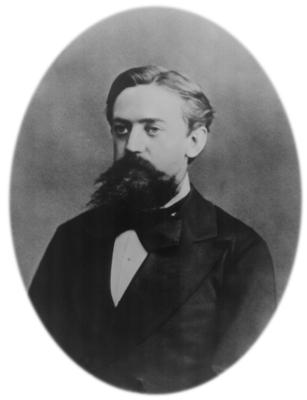
\includegraphics[height=4cm]{markov.jpg}}
\date{28.03.2013}
\institute{СПбГУ}

\begin{document}
\renewcommand*{\inserttotalframenumber}{\pageref{lastframe}}
\begin{frame}
\titlepage
\end{frame}


\begin{frame}
  \begin{itemize}
  \item Баесовская вероятность
  \item Моделирование окружающего мира и его задачи
  \item Предположение Маркова
  \item Марковские цепи
  \item HMMs
  \item Активные действия — FSMs
  \item Неуверенность в исходе: MDPs
  \item Неуверенность в измерении: POMDPs
  \end{itemize}
  \begin{center}
    HARDCORE
  \end{center}
\end{frame}

\begin{frame}
  \begin{center}
    \Large
    Баесовский взгляд на вероятность\\ aka The Red Pill
  \end{center}
\end{frame}

\begin{frame}{Классическая вероятность}
  \begin{center}
    \includegraphics[height=6cm, keepaspectratio=true]{coin_tossing.jpg}\\
    100 бросков, 53 раза решка $\implies$ P = 0.53
  \end{center}
\end{frame}

\begin{frame}{Классическая вероятность}
  \begin{center}
    \Large
    Описание окружающего мира
  \end{center}
\end{frame}

\begin{frame}{Баесовская вероятность}
  \begin{center}
  \includegraphics[height=6cm]{coin_tossing.jpg}\\
  100 бросков, 53 раза решка $\implies$ \\
  на 53\% я уверен, что выпадет решка
  \end{center}
\end{frame}

\begin{frame}{Баесовская вероятность}
  \begin{center}
    \Large
    Описание уверенности наблюдателя
  \end{center}
\end{frame}

\begin{frame}{Баесовская вероятность}
  \begin{center}
    $P(A|B) = \frac{P(B|A)P(A)}{P(B)}$
  \end{center}
  \begin{itemize}
  \item $A$ — предположение
  \item $B$ — свидетельство
  \item $P(A)$ — prior, начальная степень уверенности в А
  \item $P(A|B)$ — posterior, степень уверенности в A с учётом B
  \item $P(B|A)$ — «модель мира», вероятность B при полной уверенности в A
  \end{itemize}
\end{frame}

\begin{frame}{Баесовская вероятность: пример}
  \begin{itemize}
  \item $A$: монета честная ($\bar{A}$: монета выпадает орлом в 0.9 случаев)
  \item $B$: очередное выпадение монеты (решка=1, орёл=0)
  \item $P(A)$: начальная уверенность в честности монеты; 0.5 (uniform
    prior)
  \item $P(B|A)$: при условии честности монеты, $P(1|A)=0.5,
    P(0|A)=0.5$
  \item $P(B) = P(B|A)P(A) + P(B|\bar{A})P(\bar{A})$
  \end{itemize}
\end{frame}

\begin{frame}{Баесовская вероятность: пример}
  \begin{center}
    1
  \end{center}
  \begin{itemize}
  \item $A$: монета честная ($\bar{A}$: монета выпадает орлом в 0.9 случаев)
  \item $B$: очередное выпадение монеты (решка=1, орёл=0)
  \item $P(A)$: начальная уверенность в честности монеты; 0.5 (uniform
    prior)
  \item $P(B|A)$: при условии честности монеты, $P(1|A)=0.5,
    P(0|A)=0.5$
  \item $P(B) = P(B|A)P(A) + P(B|\bar{A})P(\bar{A})$
  \item $P(A|1)=\frac{0.5 * 0.5}{0.5 * 0.5 + 0.1 * 0.5} = 0.833$
  \end{itemize}
\end{frame}

\begin{frame}{Баесовская вероятность: пример}
  \begin{center}
    1 1
  \end{center}
  \begin{itemize}
  \item $A$: монета честная ($\bar{A}$: монета выпадает орлом в 0.9 случаев)
  \item $B$: очередное выпадение монеты (решка=1, орёл=0)
  \item $P(A)$: начальная уверенность в честности монеты; 0.833 (новый
    prior)
  \item $P(B|A)$: при условии честности монеты, $P(1|A)=0.5,
    P(0|A)=0.5$
  \item $P(B) = P(B|A)P(A) + P(B|\bar{A})P(\bar{A})$
  \item $P(A|1)=\frac{0.5 * 0.83}{0.5 * 0.83 + 0.1 * 0.17} = 0.96$
  \end{itemize}
\end{frame}

\begin{frame}{Баесовская вероятность: пример}
  \begin{center}
    1 1 1
  \end{center}
  \begin{itemize}
  \item $A$: монета честная ($\bar{A}$: монета выпадает орлом в 0.9 случаев)
  \item $B$: очередное выпадение монеты (решка=1, орёл=0)
  \item $P(A)$: начальная уверенность в честности монеты; 0.96 (новый
    prior)
  \item $P(B|A)$: при условии честности монеты, $P(1|A)=0.5,
    P(0|A)=0.5$
  \item $P(B) = P(B|A)P(A) + P(B|\bar{A})P(\bar{A})$
  \item $P(A|1)=\frac{0.5 * 0.96}{0.5 * 0.96 + 0.1 * 0.04} = 0.99$
  \end{itemize}
\end{frame}

\begin{frame}{Баесовская вероятность: пример}
  \begin{itemize}
  \item баесовский взгляд на вероятность использует «уверенность»
    (belief)
  \item наблюдения за окружающим миром меняют уверенность
  \item правило Баеса характеризует процесс обучения
  \end{itemize}
\end{frame}

\begin{frame}
  \begin{center}
    \Large
    Моделирование окружающего мира
  \end{center}
\end{frame}

\begin{frame}{Мир дождя}
  \begin{center}
      \begin{tikzpicture}[node distance=0.25cm]
    \node (day0) []
          {$\dots$};
    \node (day1) [var] [right=of day0]
          {$Rainy_{t-2}$};
    \node (day2) [var] [right=of day1]
          {$Rainy_{t-1}$}
          edge [<-,bend left] (day1);
    \node (day3) [var] [right=of day2]
          {$Rainy_{t}$}
          edge [<-,bend left] (day1)
          edge [<-,bend right] (day2);
    \node (day4) [var] [right=of day3]
          {$Rainy_{t+1}$}
          edge [<-,bend left] (day1)
          edge [<-,bend right] (day2)
          edge [<-,bend right,in=200,out=345] (day3);
    \node (day_next) [] [right=of day4]
          {$\dots$};
  \end{tikzpicture}\\
  \vspace{1em}
  $P(Rainy_t)=P(Rainy_t|Rainy_{t-1}, Rainy_{t-2}, Rainy_{t-3},
  \dots)$\\
  \vspace{1em}
  \Large
  Мир боли и унижения
  \end{center}
\end{frame}

\begin{frame}{Марков спешит на помощь!}
  \begin{center}
    Предположение Маркова (Markov assumption):\\
    \vspace{1em}
    \Large
    текущее состояние зависит от конечного
    фиксированного количества предыдущих состояний
  \end{center}
\end{frame}

\begin{frame}{Мир дождя, попытка 2}
  \begin{center}
      \begin{tikzpicture}[node distance=0.25cm]
    \node (day0) []
          {$\dots$};
    \node (day1) [var] [right=of day0]
          {$Rainy_{t-2}$};
    \node (day2) [var] [right=of day1]
          {$Rainy_{t-1}$}
          edge [<-,bend right] (day1);
    \node (day3) [var] [right=of day2]
          {$Rainy_{t}$}
          edge [<-,bend right] (day2);
    \node (day4) [var] [right=of day3]
          {$Rainy_{t+1}$}
          edge [<-,bend right] (day3);
    \node (day_next) [] [right=of day4]
          {$\dots$};
  \end{tikzpicture}
  \\
  \vspace{1em}
  $P(Rainy_t)=P(Rainy_t|Rainy_{t-1})$\\
  \vspace{1em}
  \Large
  Марковская цепь 1 порядка
  \end{center}
\end{frame}

\begin{frame}{Мир дождя, попытка 2}
  \begin{center}
    \begin{tikzpicture}[node distance=0.25cm]
    \node (day0) []
          {$\dots$};
    \node (day1) [var] [right=of day0]
          {$Rainy_{t-2}$};
    \node (day2) [var] [right=of day1]
          {$Rainy_{t-1}$}
          edge [<-,bend left] (day1);
    \node (day3) [var] [right=of day2]
          {$Rainy_{t}$}
          edge [<-,bend left] (day1)
          edge [<-,bend right] (day2);
    \node (day4) [var] [right=of day3]
          {$Rainy_{t+1}$}
          edge [<-,bend right] (day2)
          edge [<-,bend right,in=200,out=345] (day3);
    \node (day_next) [] [right=of day4]
          {$\dots$}
    \end{tikzpicture}
    \\
    \vspace{1em}
    $P(Rainy_t)=P(Rainy_t|Rainy_{t-1}, Rainy_{t-2})$\\
    \vspace{1em}
    \Large
    Марковская цепь 2 порядка
  \end{center}
\end{frame}

\begin{frame}{Мир дождя: зачем, что, почём}
  \begin{center}
      \begin{tikzpicture}[node distance=0.25cm]
    \node (day0) []
          {$\dots$};
    \node (day1) [var] [right=of day0]
          {$Rainy_{t-2}$};
    \node (day2) [var] [right=of day1]
          {$Rainy_{t-1}$}
          edge [<-,bend left] (day1);
    \node (day3) [var] [right=of day2]
          {$Rainy_{t}$}
          edge [<-,bend left] (day1)
          edge [<-,bend right] (day2);
    \node (day4) [var] [right=of day3]
          {$Rainy_{t+1}$}
          edge [<-,bend right] (day2)
          edge [<-,bend right,in=200,out=345] (day3);
    \node (day_next) [] [right=of day4]
          {$\dots$};
  \end{tikzpicture}
  \\
  \vspace{1em}
  $P(Rainy_t)=P(Rainy_t|Rainy_{t-1}, Rainy_{t-2})$\\
  \vspace{1em}
  \end{center}
  Зачем всё это?
  \begin{itemize}
  \item обучение: $P(Rainy_t|Rainy_{t-1}, Rainy_{t-2}) =
    \frac{c(Rainy_t, Rainy_{t-1}, Rainy_{t-2})}
         {c(Rainy_{t-1}, Rainy_{t-2})}$
  \item предсказание: $argmax(P(X|Rainy_{t-1}, Rainy_{t-2}))$
  \item объяснение: $argmax(P(Rainy_t|Y, Z))$
  \end{itemize}
\end{frame}

\begin{frame}{Мир лягушки}
  \begin{center}
    \begin{tikzpicture}[node distance=0.5cm]
    \node (node11) [frogpos]
          {$1$};
    \node (node12) [frogpos] [right=of node11]
          {$2$}
          edge [<->,draw=black!50] (node11);
    \node (node13) [frogpos] [right=of node12]
          {$3$}
          edge [<->,draw=black!50] (node12);
    \node (node21) [frogpos] [below=of node11]
          {$4$}
          edge [<->,draw=black!50] (node11);
    \node (node22) [frogpos] [right=of node21]
          {$5$}
          edge [<->,draw=black!50] (node21)
          edge [<->,draw=black!50] (node12);
    \node (node23) [frogpos] [right=of node22,fill=black!20]
          {$6$}
          edge [<->, thick] (node22)
          edge [<->, thick] (node13);
    \node (node31) [frogpos] [below=of node21]
          {$7$}
          edge [<->,draw=black!50] (node21);
    \node (node32) [frogpos] [right=of node31]
          {$8$}
          edge [<->,draw=black!50] (node31)
          edge [<->,draw=black!50] (node22);
    \node (node33) [frogpos] [right=of node32]
          {$9$}
          edge [<->,draw=black!50] (node32)
          edge [<->,thick] (node23);
    \end{tikzpicture}
    \\
    \vspace{1em}
    \large
    $x \in \{1,2,\dots,9\}$\\
    $P(x) = P(x_t|x_{t-1})$\\
    \vspace{1em}
    \Large
    Марковская цепь 1 порядка
  \end{center}
\end{frame}

\begin{frame}{Мир лягушки}
  \begin{center}
    \begin{tikzpicture}[node distance=0.5cm]
    \node (node11) [frogpos]
          {$1$};
    \node (node12) [frogpos] [right=of node11]
          {$2$}
          edge [<->,draw=black!50] (node11);
    \node (node13) [frogpos] [right=of node12]
          {$3$}
          edge [<->,draw=black!50] (node12);
    \node (node21) [frogpos] [below=of node11]
          {$4$}
          edge [<->,draw=black!50] (node11);
    \node (node22) [frogpos] [right=of node21]
          {$5$}
          edge [<->,draw=black!50] (node21)
          edge [<->,draw=black!50] (node12);
    \node (node23) [frogpos] [right=of node22,fill=black!20]
          {$6$}
          edge [<->, thick] (node22)
          edge [<->, thick] (node13);
    \node (node31) [frogpos] [below=of node21]
          {$7$}
          edge [<->,draw=black!50] (node21);
    \node (node32) [frogpos] [right=of node31]
          {$8$}
          edge [<->,draw=black!50] (node31)
          edge [<->,draw=black!50] (node22);
    \node (node33) [frogpos] [right=of node32]
          {$9$}
          edge [<->,draw=black!50] (node32)
          edge [<->,thick] (node23);
    \end{tikzpicture}
    \\
    \vspace{1em}
    Матрица переходов P:\\
    \large
    \begin{array}{c|cccc}
        & 1           & 2           & 3           & \hdots \\[0.3em]
      \hline
      1 & 0           & \frac{1}{2} & 0           &        \\[0.3em]
      2 & \frac{1}{3} & 0           & \frac{1}{3} &        \\[0.3em]
      3 & 0           & \frac{1}{2} & 0           &        \\[0.3em]
      4 & \frac{1}{3} & 0           & 0           &        \\[0.3em]
      \vdots  &       &             &             &
    \end{array}
  \end{center}
\end{frame}

\begin{frame}
  \begin{center}
    \Large
    Симуляция! (frog\_sim.m, frog1.mp4, frog2.mp4)
  \end{center}
\end{frame}

\begin{frame}{Мир лягушки}
  И что?
  \begin{itemize}
  \item более сложные миры (3D)
  \item симуляция случайных процессов (броуновское движение)
  \item положение автомобиля в городе, пакета в сети, атома в
    кристаллической решётке, …
  \end{itemize}
\end{frame}

\begin{frame}
  \begin{center}
    \Large
    Hidden Markov Models (HMMs)
  \end{center}
\end{frame}

\begin{frame}{Мир дождя и зонтиков}
  \begin{center}
      \begin{tikzpicture}[node distance=0.8cm]
    \node (day0) []
          {$\dots$};
    \node (day1) [var] [right=of day0]
          {$Rainy_{t-1}$};
    \node (day2) [var] [right=of day1]
          {$Rainy_{t}$}
          edge [<-] (day1);
    \node (day3) [var] [right=of day2]
          {$Rainy_{t+1}$}
          edge [<-] (day2);
    \node (day_next) [] [right=of day3]
          {$\dots$};
    \node (umb1) [var] [below=of day1]
          {$Umbrella_{t-1}$}
          edge [<-] (day1);
    \node (umb2) [var] [below=of day2]
          {$Umbrella_{t}$}
          edge [<-] (day2);
    \node (umb3) [var] [below=of day3]
          {$Umbrella_{t+1}$}
          edge [<-] (day3);
  \end{tikzpicture}
  \\
  \vspace{1em}
  $P(Rainy_t)=P(Rainy_t|Rainy_{t-1})$ (модель мира)\\
  $P(Umbrella_t)=P(Umbrella_t|Rainy_t)$ (модель сенсоров)\\
  \vspace{1em}
  \Large
  HMM 1 порядка
  \end{center}
  \begin{itemize}
  \item истинное состояние мира неизвестно
  \item состояние мира измеряется ненадёжными сенсорами
  \end{itemize}
\end{frame}

\begin{frame}{Мир дождя и зонтиков}
  \begin{center}
      \begin{tikzpicture}[node distance=0.8cm]
    \node (day0) []
          {$\dots$};
    \node (day1) [var] [right=of day0]
          {$Rainy_{t-1}$};
    \node (day2) [var] [right=of day1]
          {$Rainy_{t}$}
          edge [<-] (day1);
    \node (day3) [var] [right=of day2]
          {$Rainy_{t+1}$}
          edge [<-] (day2);
    \node (day_next) [] [right=of day3]
          {$\dots$};
    \node (umb1) [var] [below=of day1]
          {$Umbrella_{t-1}$}
          edge [<-] (day1);
    \node (umb2) [var] [below=of day2]
          {$Umbrella_{t}$}
          edge [<-] (day2);
    \node (umb3) [var] [below=of day3]
          {$Umbrella_{t+1}$}
          edge [<-] (day3);
  \end{tikzpicture}
  \\
  \vspace{1em}
  $P(Rainy_t)=P(Rainy_t|Rainy_{t-1})$ (модель мира)\\
  $P(Umbrella_t)=P(Umbrella_t|Rainy_t)$ (модель сенсоров)\\
  \vspace{1em}
  \end{center}
  Зачем всё это?
  \begin{itemize}
  \item Наблюдается только $Umbrella_{1 \dots t}$ (с ошибкой)
  \item То же, что у простых марковских моделей (обучение,
    предсказание, объяснение)
  \item Восстановление сигнала (сигнал скрыт, известны измерения)
  \end{itemize}
\end{frame}

\begin{frame}{Пример: части речи}
  \begin{center}
    \large
    Задача: «мама мыла раму» $\iff$ |Cущ Гл Сущ STOP|
  \end{center}
\end{frame}

\begin{frame}{Пример: части речи}
  \begin{center}
  \begin{tikzpicture}[node distance=0.5cm]
    \node (s1) [var, circle, minimum size=1.1cm]
          {*};
    \node (s2) [var, circle, minimum size=1.1cm] [right=of s1]
          {*};
    \node (s3) [var, circle, minimum size=1.1cm] [right=of s2]
          {Сущ}
          edge [<-, bend right] (s1)
          edge [<-] (s2);
    \node (s4) [var, circle, minimum size=1.1cm] [right=of s3]
          {Гл}
          edge [<-, bend right] (s2)
          edge [<-] (s3);
    \node (s5) [var, circle, minimum size=1.1cm] [right=of s4]
          {Сущ}
          edge [<-, bend right] (s3)
          edge [<-] (s4);
    \node (s6) [var, circle, minimum size=1.1cm] [right=of s5]
          {STOP}
          edge [<-, bend right] (s4)
          edge [<-] (s5);
    \node (q1) [var] [below=of s3]
          {мама}
          edge [<-] (s3);
    \node (q2) [var] [below=of s4]
          {мыла}
          edge [<-] (s4);
    \node (q3) [var] [below=of s5]
          {раму}
          edge [<-] (s5);
  \end{tikzpicture}
  \\
  \vspace{1cm}
  \end{center}
  \begin{itemize}
  \item HMM 2 порядка
  \item P(раму|Сущ)$, $P(мыла|Гл)$, $P(мыла|Сущ)$, $P(Сущ|Гл, Сущ), …
  \item |Сущ Гл Сущ STOP| — наиболее вероятная цепочка, объясняющая «мама мыла
  раму»
  \item $argmax(P(x_1, x_2, \dots, x_n, y_1, y_2, \dots, y_m))$
  \end{itemize}
\end{frame}


\begin{frame}
  \begin{center}
    \Large
    Конечные автоматы
  \end{center}
\end{frame}

\begin{frame}{Конечный автомат}
  \begin{center}
    \begin{tikzpicture}[node distance=5cm]
    \node (door_open) [var, circle]
          {Дверь открыта};
    \node (door_closed) [var, circle] [below left of=nodea]
          {Дверь закрыта}
          edge [<-, bend left] node[left] {Закрыть дверь} (door_open)
          edge [->, bend right] node[right] {Открыть дверь} (door_open);
    \node (lock_closed) [var, circle] [below right of=nodea]
          {Замок закрыт}
          edge [<-, bend left] node[below] {Закрыть замок} (door_closed);
  \end{tikzpicture}
  \end{center}
\end{frame}

\begin{frame}{Мир пылесоса}
  \begin{center}
    Мир:\\
    \begin{tikzpicture}[node distance=2.3cm]
    \node (left_room) [rectangle, draw=black,very thick,
                       minimum size=1.5cm]
          {L};
    \node (right_room) [rectangle, draw=black,very thick,
                        minimum size=1.5cm]
                       [right of=left_room]
          {R}
          edge [<->, very thick] (left_room);
  \end{tikzpicture}
  \\
  \vspace{0.5cm}
  Конечный автомат:\\
  \begin{tikzpicture}[node distance=2.5cm]
    \node (l) [var, circle]
          {L};
    \node (r) [var, circle] [right of=l,xshift=2cm]
          {R}
          edge [->, bend left] node[above] {Move L} (l)
          edge [<-, bend right] node[below] {Move R} (l);
    \node (LS) [var, circle] [below of=l]
          {L, Suck}
          edge [<-, bend left] node[left] {Suck} (l)
          edge [->, bend right] node[right] {Stop} (l);
    \node (RS) [var, circle] [below of=r]
          {R, Suck}
          edge [<-, bend left] node[left] {Suck} (r)
          edge [->, bend right] node[right] {Stop} (r);
  \end{tikzpicture}
  \end{center}
\end{frame}

\begin{frame}
  \begin{center}
    \Large
    Markov Decision Processes (MDPs),\\
    Partially Observable MDPs (POMPDs)
  \end{center}
\end{frame}

\begin{frame}{Мир глючного пылесоса}
  \begin{center}
  \begin{tikzpicture}[node distance=2.5cm]
    \node (l) [var, circle]
          {L};
    \node (lm) [var, circle, fill=black!20] [right of=l, xshift=-0.5cm]
          {Move R}
          edge [<-] (l)
          edge [->, bend right] node[above] {0.1} (l);
    \node (rm) [var, circle, fill=black!20] [right of=lm, xshift=1cm]
          {Move L}
          edge [->, bend left] node[below] {0.9} (lm)
          edge [<-, bend right] node[above] {0.9} (lm);
    \node (r) [var, circle] [right of=rm, xshift=-0.5cm]
          {R}
          edge [->] (rm)
          edge [<-, bend right] node[above] {0.1} (rm);
    \node (LS) [var, circle] [below of=l]
          {L, Suck}
          edge [<-, bend left] node[left] {Suck} (l)
          edge [->, bend right] node[right] {Stop} (l);
    \node (RS) [var, circle] [below of=r]
          {R, Suck}
          edge [<-, bend left] node[left] {Suck} (r)
          edge [->, bend right] node[right] {Stop} (r);
  \end{tikzpicture}
  \\
  \vspace{1cm}
  \large
  Действия не всегда приводят к ожидаемому результату
  \end{center}
\end{frame}

\begin{frame}{Обобщим}
  \begin{center}
    \begin{tabular}{ l | c c c }
       Управление:   & Состояние: & известно & неизвестно \\
       \hline
       нет  & & Цепь Маркова         & HMMs                   \\
       есть & & MDPs                 & POMDPs                 \\
    \end{tabular}
  \end{center}
  \begin{itemize}
  \item самая важная часть презентации $\uparrow$
  \item везде используется предположение Маркова
  \item посмотрим на цепи, HMMs и MDPs ещё раз
  \end{itemize}
\end{frame}

\begin{frame}
  \begin{center}
    \Large
    Спасибо за внимание!\\
    \vspace{1cm}
    \small
    \url{https://github.com/si14/uni-prob-markov-2013-03/}
  \end{center}
\end{frame}

\begin{frame}\label{lastframe}
  \footnotesize
  Использовались картинки:
  \begin{itemize}
    \item \url{http://en.wikipedia.org/wiki/File:Coin_tossing.JPG}
    \item \url{http://commons.wikimedia.org/wiki/File:AAMarkov.jpg}
  \end{itemize}
\end{frame}
